% ==================================================
% CHAPTER 1: Introduction %
% ==================================================

\chapter{Introduction}
\label{chap:intro}
% Edit count: Lia - 0, Brigitte - 0

% Miscellaneous intros
%The Large Hadron Collider (LHC) and the ATLAS experiment were designed to search for a Higgs boson~\cite{atlas_letter_of_intent_1992}
%The primary goal in building the Large Hadron Collider (LHC) and the ATLAS experiment was to search for a Higgs boson
%Studying particle detectors is interesting because of the interplay between the physics of what is to be studied with the detector and the physics of how the detector works. 
%Particle detectors intertwine physics concepts at multiple scales since their use requires understanding both the physics of how they work and the physics of what they are meant to study. 
%The details of how a particle detector works intertwine with the physics it is meant to study. Especially in a collaboration as large as ATLAS. 
%Small-strip thin gap chambers (sTGCs) for the ATLAS experiment at CERN 
%The questions proposed in the first recorded physics case for the Large Hadron Collider (LHC) are still only partially answered~\cite{brianti_large_1984}. it is clear there is still more to study at the LHC if the study of the %standard model is to continue. 
%The High-Lumnosity Large Hadron Collider (HL-LHC) project was approved to combat the plateau in statistial gain of recording particle collisions at the LHC at CERN~\cite{hl_lhc_tdr}. 
%The questions proposed in the first recorded physics case for the Large Hadron Collider (LHC) are still only 
%If the study of particle physics is to continue, studying the Higgs boson 

% --------------------------------------------------
\section{Introduction}
% --------------------------------------------------

THIS IS REALLY ROUGH. BASED ON ALESSANDRO'S IDEA OF SHOWING THE FULL INTRO OVERVIEW THEN DIVING INTO ALL THE NECESSARY DETAILS.

The High-Lumnosity Large Hadron Collider (HL-LHC) project was approved to combat the plateau in statistial gain of recording particle collisions at the LHC at CERN~\cite{hl_lhc_tdr}. Being the most energetic particle accelerator, the LHC still offers unique physics opportunities for studying the Higgs and electroweak sectors of the standard model; if the study of the standard model is to continue, the LHC must go on. The HL-LHC upgrade aims to increase the luminosity of the LHC by up to a factor of 7 in the next 10 years, which ultimately increases the number of meaningful collisions. Naturally, various sub-systems of the experiments used to capture the outcomes of the collisions will require upgrades to handle higher collision rates and background radiation rates than they were designed for. 

The ATLAS experiment is one of the LHC's general-purpose particle detector arrays. The largest upgrade the ATLAS experiment will undergo is the replacement of the small wheels of the muon spectrometer with the so-called New Small Wheels (NSWs). Two different detector technologies will be installed: micromegas, and small-strip thin gap chambers (or sTGCs). In this work, the dataset used to correct for the internal alignment of sTGC components is validated with characterization data collected on the sTGCs using cosmic muons. How the internal alignment fits into the overall alignment system is also detailed. 

Information necessary to understand the ATLAS detector, the NSW upgrade, sTGCs and the NSW alignment system is presented in this chapter. 

% --------------------------------------------------
\section{The Large Hadron Collider}
% --------------------------------------------------

% Include order for inst lum.
% Include bunch crossing frequency
The LHC is an accelerator \SI{27}{\kilo\meter} in circumference and located $\sim$\SI{100}{\meter} underground at CERN near Geneva, Switzerland~\cite{evans_lhc_2008}. It has two beam pipes that counter-circulate bunches of protons\footnote{the LHC also accelerates lead ions, but this paper only considers proton-proton collisions} before colliding the bunches in the center of one of four major experiments, such as the ATLAS experiment (discussed in section~\ref{sec:atlas}). There, the partons interact and many physics processes can occur. The LHC enables physicists to study particle physics at the energy frontier. In the previous run of the LHC (run 2), protons were collided with a center of mass energy of \SI{13}{\tera\electronvolt}. 

% There are two main branches of study that can be pursued with the LHC and ATLAS. First, properties predicted by the standard model (SM) of particle physics can be measured. Else, physicists can search for evidence of processes predicted by theories beyond the standard model. Both the SM measurement and search analyses are based on measuring the number of times a given process occurs and comparing it to expectations. In this way, the number of proton-proton interactions created by the LHC directly affects the statistics available to do SM measurements and searches using the ATLAS experiment.


The number of proton-proton interactions generated by the LHC directly affects the statistics available to make fundamental measurements of cross sections, event rates, etc. 
%IF YOU DON'T NEED TO DEFINE LUMINOSITY
% The number of interactions is quantified by luminosity, a property of the accelerator and its operating conditions~\cite{zyla_review_2020}. When the instantaneous luminosity is integrated over a data collection period and multiplied by the cross section of a given process, the result is the expected number of times that process occurs (so luminosity has units of inverse cross section). Since luminosity is derived from the accelerator parameters, it is the link between the machine and the statistical power of potential measurements. 
% IF YOU NEED TO DEFINE LUMINOSITY
% THIS SECTION IS NOT CITED, probably cite wiht zyla_review_2020
Predicting the number of proton-proton interactions requires defining a metric called luminosity~\cite{zyla_review_2020}. It is the number of particles an accelerator can send through a given area per unit time. It is calculated from the measurable quantities in equation~\ref{eqn:inst_lum}.

\begin{equation}
\mathcal{L} = \frac{f N_{1} N_{2} }{4 \pi \sigma_{x} \sigma_{y}}
\label{eqn:inst_lum}
\end{equation}

In equation~\ref{eqn:inst_lum}, $f$ is the frequency of the bunch crossings (\SI{25}{\nano\second}), $N_{1}$ and $N_{2}$ are the number of protons in each bunch ($\sim 10^{11}$ protons / bunch), and $\sigma_{x}$ and $\sigma_{y}$ are the RMS of the spatial distributions of the bunch; therefore, luminosity is a property of the accelerator and its operating parameters. The design luminosity of the LHC was $10^{34}$ cm$^{-2}$s$^{-1}$. Multiplying the luminosity by the cross section of a given process gives the expected rate for that process.

Integrating the \textit{instantaneous} luminosity (equation~\ref{eqn:inst_lum}) over a period of data collection gives the integrated luminosity,

\begin{equation}
L = \int \mathcal{L} \left( t \right) \,dt
\label{eqn:int_lum}
\end{equation}

with units of an inverse cross section and related to the total number of interactions. In this way, the luminosity is the link between the accelerator and the statistical power of measurements to be made with the data collected. 

So far, the LHC provided an integrated luminosity of \SI{30}{\per\femto\barn} in run 1 and \SI{190}{\per\femto\barn} in run 2, as shown in figure~\ref{fig:hl-lhc}. The HL-LHC upgrade~\cite{hl_lhc_tdr} \textcolor{red}{(this will be discussed earlier in the introduction)} was accepted because without increasing the luminosity of the LHC tenfold, running the accelerator will not provide significant statistical gain on measurements. Also, some systems will need repair and replacement to operate past $\sim$2020. The energy accessible at the LHC offers irreplaceable ability to study Higgs- and electroweak-sector physics~\cite{dainese_physics_2018}, so the European Strategy for Particle Physics made it a priority ``to fully exploit the physics potential of the LHC'' with ``a major luminosity upgrade''~\cite{european_strategy_for_particle_physics}. The goal is for the LHC to provide an integrated luminosity\SI{3000}{\per\femto\barn} in the 12 years following the upgrade. The luminosity actually achieved will depend on a combination of technological advances and upgrades in progress~\cite{hl_lhc_tdr} that affect the factors contributing to luminosity defined in equation~\ref{eqn:inst_lum}.


\begin{figure}
    \centering
    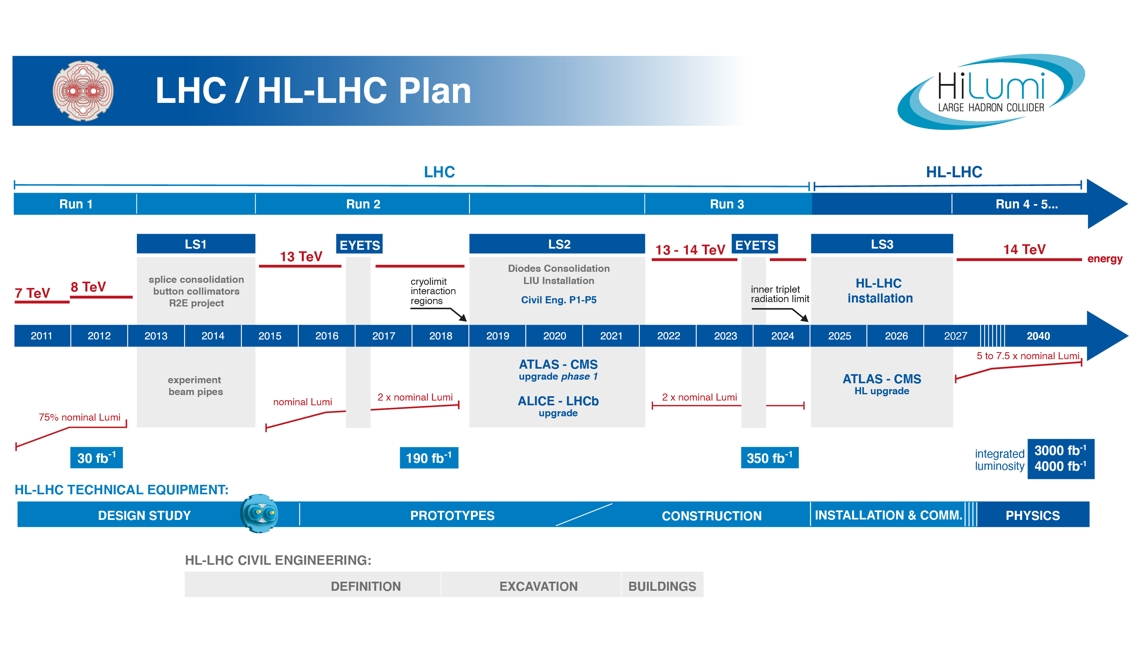
\includegraphics[width = \textwidth]{figures/HL-LHC-updated-January-2021_small.jpg}
    \caption{LHC/HL-LHC plan~\cite{hl-lhc_plan_picture_website}. The integrated luminosity collected and projected for each run of the LHC is shown in red below the timeline. The center of mass energy of the collisions is shown in red above the timeline. ``LS'' stands for ``long shutdown'' and indicates periods where the accelerator is not operating. During the shutdowns, upgrades to the LHC and the experiments are being installed. This timeline was last updated in January, 2021, and reflects changes in the schedule due to the ongoing pandemic. }
    \label{fig:hl-lhc}
\end{figure}

%The estimated number of interactions of a given type per bunch crossing is given by equation~\ref{eqn:num_interactions}.
%\begin{equation}
%\mu = \sigma \delta t\mathcal{L}
%\label{eqn:num_interactions}
%\end{equation}

% The energies accessible by the accelerator make it unique infrastructure with which to study processes of the standard model of particle physics and search for new phenomenon beyond the standard
% model. Considerable progress has been made towards answering the questions originally used to motivate the construction of the LHC, but many remain unanswered or only partially answered~ \cite{brianti_large_1984}. Therefore, the continued use and maintenance of the accelerator 

% --------------------------------------------------
\section{The ATLAS experiment}
% --------------------------------------------------
\label{sec:atlas}

The ATLAS experiment~\cite{collaboration_atlas_2008} was designed to support all the physics goals of the LHC. It is \SI{44}{\meter} long and \SI{25}{\meter} in diameter, and weighs 7000 tones. It is an array of particle detector subsystems arranged concentrically around the beam pipe and centered around one of the LHC's interaction points (a place where the beams collide), as shown in figure~\ref{fig:atlas}. It is helpful to separate the subsystems of ATLAS into the so-called ``barrel'' and ``encap'' (or forward region), referring to the cylindrical shape.  % <- maybe move this sentence to muon spec section

\begin{figure}
    \centering
    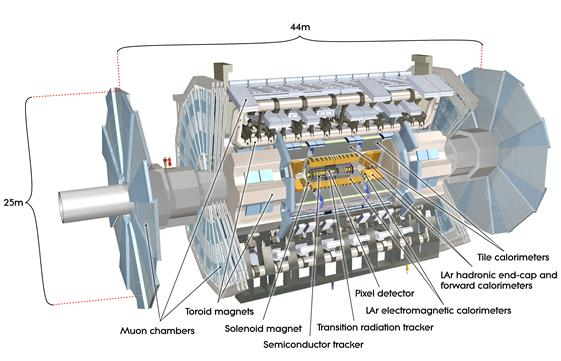
\includegraphics[width = \textwidth]{figures/atlas_diagram.png}
    \caption{Diagram of the ATLAS experiment, with the various detector subsystems labelled. Figure from~\cite{collaboration_atlas_2008}, which also contains more details about the ATLAS experiment.}
    \label{fig:atlas}
\end{figure}

For analysis, ATLAS is typically described in spherical coordinates. The azimuthal angle $\phi$ is measured around the beampipe and the polar angle $\theta$ is measured from the beam pipe. A more useful coordinate than $\theta$ is the pseudo-rapidity, $\eta = -\ln\tan\left(\theta/2\right)$, because it approaches the rapidity of a particle when its momentum is much greater than its mass and differences in rapidity are approximately invariant to a Lorentz boost parallel to the beam. The range of $\eta$ is 0 (perpendicular to the beam) to $\pm\inf$ (parallel to the beam). Typically, $\eta$ is the physically interesting coordinate because the $\phi$ coordinate follows the cylindrical symmetry.

It is not actually the proton bunches that collide and generate physics processes, but their constituent partons. Since the partons may carry an unknown fraction of the momentum, ATLAS analyses are based on the sum of the transverse momentum and energy of outgoing particle being approximately zero, transverse meaning perpendicular to the beam. The goal of ATLAS is to reconstruct the 4-momentum of each collision product to understand what happened in each collision. A brief overview of the sub-systems of ATLAS is given, starting from the system closest to the beam and moving outwards. 

\textbf{The inner detector}

The inner detector~\cite{atlas_inner_detector_tdr_1, atlas_inner_detector_tdr_2} (figure~\ref{fig:atlas_inner_detector}) is for precision tracking, vertex measurements and electron identification. A \SI{2}{\tesla} solenoid with field parallel to the beam bends the track of outgoing particles to make momentum measurements possible. The innermost part is made of high-resolution semiconductor pixel and strip detectors for precision tracking while the outermost part are straw-tubes that generate and detect transition radiation for electron identification.

\begin{figure}
    \centering
    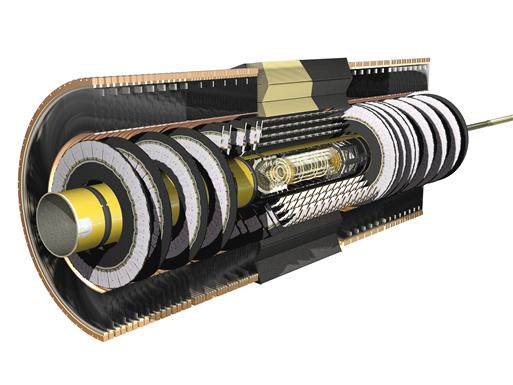
\includegraphics[width = 0.5\textwidth]{figures/atlas_inner_detector.jpg}
    \caption{Diagram of the ATLAS experiment's inner detector, with the different segments and the technology used labelled. Figure from~\cite{collaboration_atlas_2008}.}
    \label{fig:atlas_inner_detector}
\end{figure}

\textbf{Calorimeters}

Electromagnetic and hadronic sampling calorimeter units are used to record the energy of electrons, photons, jets and missing transverse energy (from neutrinos, for example). A combination of liquid-argon electromagnetic and hadronic calorimeters~\cite{atlas_lar_cal_tdr} and tile-scintillator hadronic calorimeters~\cite{atlas_tile_cal_tdr} cover the rapidity range $|\eta| < 4.9$, as shown in figure~\ref{fig:atlas_calorimeter}.

\begin{figure}
    \centering
    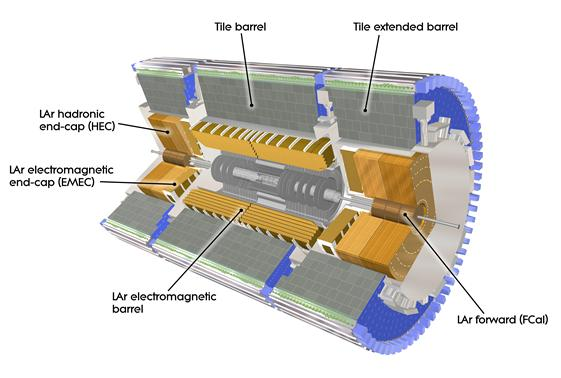
\includegraphics[width = 0.5\textwidth]{figures/atlas_calorimeter.png}
    \caption{Diagram of the ATLAS calorimeter system, with the different segments and the technology used labelled. Figure from~\cite{collaboration_atlas_2008}.}
    \label{fig:atlas_calorimeter}
\end{figure}

The calorimeters cause incoming charged particles to shower and deposit their energy in the sensitive volume. Only muons and neutrinos are known to pass the calorimeters to the muon spectrometer.  Particles other than those mentioned would have decayed in the inner detector before reaching the calorimeter. 

\textbf{Triggering}

It would be impossible to record all the data from bunch crossings every \SI{25}{\nano\second} at a rate of $\sim$\SI{40}{MHz}, so ATLAS has a multi-level trigger system to select events of interest and unambiguously assign them a to a bunch crossing. The Level-1 (L1) hardware trigger uses partial-granularity information from the muon spectrometer and calorimeter to trigger on high $p_T$ muons, electrons, jets, high missing transverse energy, and $\tau$ decaying to hadrons. The maximum L1 trigger rate ATLAS can accommodate is \SI{100}{kHz} with a latency of \SI{2.5}{\micro\second}~\cite{atlas_l1_trigger_tdr}. 

% The Level-1 (L1) hardware trigger uses the muon spectrometer's TGCs and RPCs to trigger on high $p_T$ muons and the calorimeter detector units to trigger on electrons, jets, high missing transverse energy, and $\tau$ decaying to hadrons, with a maximum trigger rate of \SI{100}{kHz} and latency of \SI{2.5}{\micro\second}. The L1 trigger only uses a fraction of the granularity offered by the detectors.

The L1 trigger is used to define regions of interest that are fed into the software high level trigger (HLT), in which the full granularity of the muon spectrometer and calorimeter are used with information from the inner detector to reduce the trigger rate to 1 kHz. Events that pass the L1 and HLT trigger are recorded for use in offline analysis~\cite{atlas_hlt_trigger_tdr}.

The ATLAS trigger system is described in the references above but the trigger rates quoted here are after the upgrades implemented for run 2, described in~\cite{martinez_run-2_2016}.

\textbf{The ATLAS muon spectrometer}

Magnetic deflection by superconducting air-core toroid magnets is used to measure muon momentum and energy. In the barrel of ATLAS, eight coils bent into ``racetracks'' are arranged around the beampipe provide the magentic field. In the forward region, two end-cap toroids each with eight smaller racetrack-shaped coils arranged symmetrically around the beampipe are inserted in the ends of the barrel toroid. Figure~\ref{fig:atlas_muon_spectrometer} shows the toroid magnets and the different parts of the ATLAS muon spectrometer.

\begin{figure}
\centering
\begin{subfigure}{.5\textwidth}
  \centering
  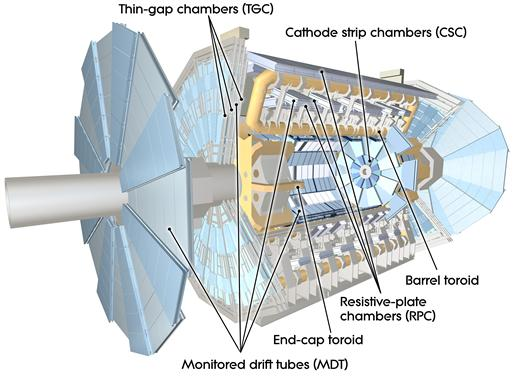
\includegraphics[width=\linewidth]{figures/atlas_muon_spectrometer.jpg}
  \caption{}
  \label{fig:atlas_muon_spectrometer_3D}
\end{subfigure}%
\begin{subfigure}{.5\textwidth}
  \centering
  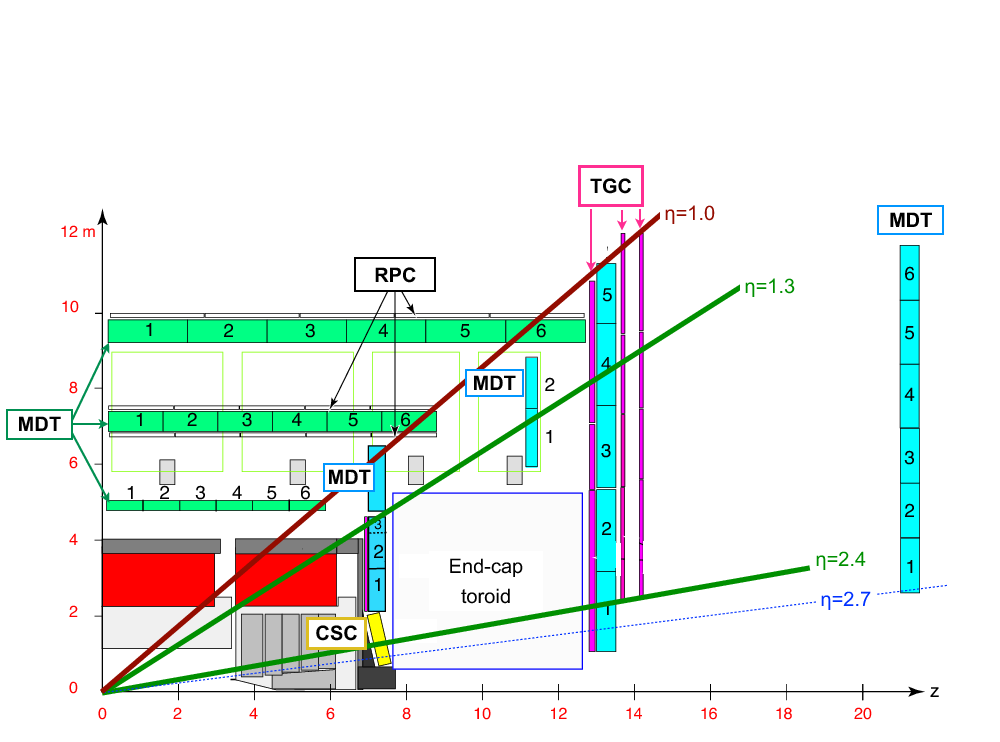
\includegraphics[width=\linewidth]{figures/atlas_old_muon_spec_quarter_cut_recolour.png}
  \caption{}
  \label{fig:atlas_muon_spectrometer_cut}
\end{subfigure}
\caption{(a) The ATLAS muon spectrometer~\cite{collaboration_atlas_2008}. (b) A quarter-cut of ATLAS, with the interaction point in the bottom left corner. The small wheel is just left of the end cap toroid, the big wheel is to its right, and the outer wheel is the rightmost structure~\cite{atlas_performance_muon_trigger_2015}}
\label{fig:atlas_muon_spectrometer}
\end{figure}

The muon spectrometer is separated into detectors used for precision offline tracking and for triggering. Monitored drift tubes (MDTs) and cathode strip chambers (CSCs) are used for precision tracking; resistive plate chambers (RPCs) are used for triggering in the barrel and thin-gap chambers (TGCs) are used for triggering in the endcaps. The positions of each type of chamber are sketched in figure~\ref{fig:atlas_muon_spectrometer_cut}. 

Precision tracking is done offline for events passing the muon trigger. Each of the barrel and encap systems have three layers of MDT that record the position of the muon as it passes through each layer. Knowing the magentic field, the muon's momentum can then be extracted. For the design momentum resolution of $\Delta p_T / p_T < 1\times10^{-4}~p / GeV$ for $p_T < 300 GeV$ and a few percent for lower $p_T$ muons, the MDTs and CSCs required position resolution of \SI{50}{\micro\meter} each. Accordingly, an optical alignment system was designed to monitor and correct for chamber positions~\cite{atlas_muon_spectrometer_tdr, aefsky_optical_2008}. 

% ON MUON TRIGGERING IN THE ENDCAP
% Decide how you want to do this based on the next section.
% At least 2 TGC layers in coincidence comes from muon spectrometer TDR; coincidence with "forward inner" detectors (small wheel) comes from run 2 trigger upgrades paper, Martinez.
% NSW TDR says there are TGC layers in the small wheel that are the forward inner detectors added to run 2 triggering.
% \textcolor{red}{The run 2 L1 muon trigger was passed if TGC layers (two for low $p_T$ muons, three for high $p_T$ muons) of the big wheel fired in coincidence with a hit from the MDTs of the small wheel on the order of the bunch crossing time. The regions of interest defined by the TGCs were fed into the HLT, where MDT and TGC data could be combined for further cuts. The $p_T$ resolution of the L1 trigger is improved by the MDT tracking information. \textit{I'll decide how I want to do this after writing the motivation for the NSW}}
In run 1, low (high) $p_T$ muons were triggered on at L1 if two (three) of the RPCs or TGCs layers fired in coincidence, for the barrel and encaps respectively~\cite{atlas_l1_trigger_tdr}. After run 1 it was discovered that up to 90\% of the triggers in the endcap were fake, caused by background particles generated in the material between the small wheel and the big wheel~\cite{nsw_tdr}. In run 1, only the TGC layers surrounding the big wheel were included in the trigger. To reduce the fake rate in run 2, the TGCs on the inside of the small wheel were also included. The added condition reduced the trigger rate by 50\% in the range 1.3 $< |\eta| <$ 1.9~\cite{martinez_run-2_2016}. The effectiveness of the solution was limited since the $|\eta|$-range of the small wheel TGC is limited to 1.0 $< |\eta| <$ 1.9 and the position resolution of the small wheel TGC doublet is coarse~\cite{nsw_tdr}.

% In the barrel, three layers of MDTs are used for precision tracking, and resistive plate chambers (RPCs) are used for triggering. The endcaps of the muon spectrometer are composed of three wheels each, the small wheel (SW), big wheel, and outer wheel. All three wheels use MDTs for precision offline tracking, but cathode strip chambers (CSCs) are used in the forward region of the small wheel because they can better handle the increased background. Thin gap  chambers

% The big wheel and the outer wheel have MDTs for offline precision tracking and the thin gap chambers (TGCs) on either side for triggering. In the first two runs of ATLAS, offline precision tracking on the small wheel was done with MDTs and cathode strip chambers (CSCs), and their output did not contribute to the trigger.~\cite{atlas_muon_spectrometer_tdr}. 

% Sentences if you go without 1/4 cut figure
% In the barrel, three layers of monitored drift tubes (MDTs) are arranged between, above and below the barrel toroid magnets. They are used for precision tracking. On both sides of the middle layer of  MDTs and on the top of the top layer of MDTs are resitive plate chambers (RPCs), used for triggering.
%  The inner part had cathode strip chambers (CSCs), which had higher granularity to handle the increased background radiation rate in the forward region

% The muon spectrometer is the outermost layer of the ATLAS detector, since only muons (and neutrinos) can pass through the calorimeters. For muons that are ejected towards the end-caps of ATLAS, their trajectory is bent by the magentic field and their position recorded by three successive wheels of muon detectors. With each wheel providing the position of the muon along its trajectory and knowledge of the magentic field, the momentum of the muon generated in the collision can be reconstructed. 

% --------------------------------------------------
\section{Motivation for the New Small Wheels (NSWs)}
% --------------------------------------------------

At the end of the HL-LHC upgrade, there could be up to a sevenfold increase in luminosity. Simultaneously, the background radiation rate increases linearly with luminosity, presenting problems for both the tracking and triggering capabilities of the muon spectrometer.

In term of tracking, the efficiency of the MDTs decreases by 35\% (mostly due to long dead-times) already when exposed to the maximum hit rate at the current luminosity, 300 kHz.
At a threefold increase in luminosity, which is predicted for run 3, most of the SW will be subjected to a hit rate well above 300 kHz. Losing muon hits in the small wheel will reduce the high $p_T$ muon momentum resolution. The decrease in resolution will affect the ability to search for high mass $Z'$, $W'$ and pseudo-scalar Higgs.

Already, the forward muon trigger system copes with a very high fake rate, even when including TGC data from the SW in the trigger as in run 2. At the luminosity expected in run 3, 60 kHz of the maximum 100 kHz of the L1 trigger would be taken by the endcap muon spectrometer. A possible solution would be to raise the minimum $p_T$ threshold from \SI{20}{\giga\electronvolt} to \SI{40}{\giga\electronvolt}, but the ability to study several physics processes of interest depend on low $p_T$ muons.

%TODO : What position resolution is nominal now? 
The NSW will solve both these problems. It will be covered with precision tracking chambers suitable for the expected hit rates and triggering chambers capable of 1 mrad angular resolution. The idea behind the triggering chambers is to match the small wheel track segment with the track segment from the big wheel to discard tracks not originating from the interaction point. Figure~\ref{fig:nsw_track_triggering} illustrates this point: the old trigger system would have triggered on all three tracks, while with the NSW the trigger system would only trigger on track A~\cite{nsw_tdr}.

% Currently, the small wheel is made of thin-gap chambers, which record hits. They have the known problem that particles generated in the material of the end-cap toroid magnet that hit the small wheel cannot be distinguished from muons from the interaction point. For example, in figure~\ref{fig:nsw_track_triggering}, all three tracks would be triggered on.

\begin{figure}
    \centering
    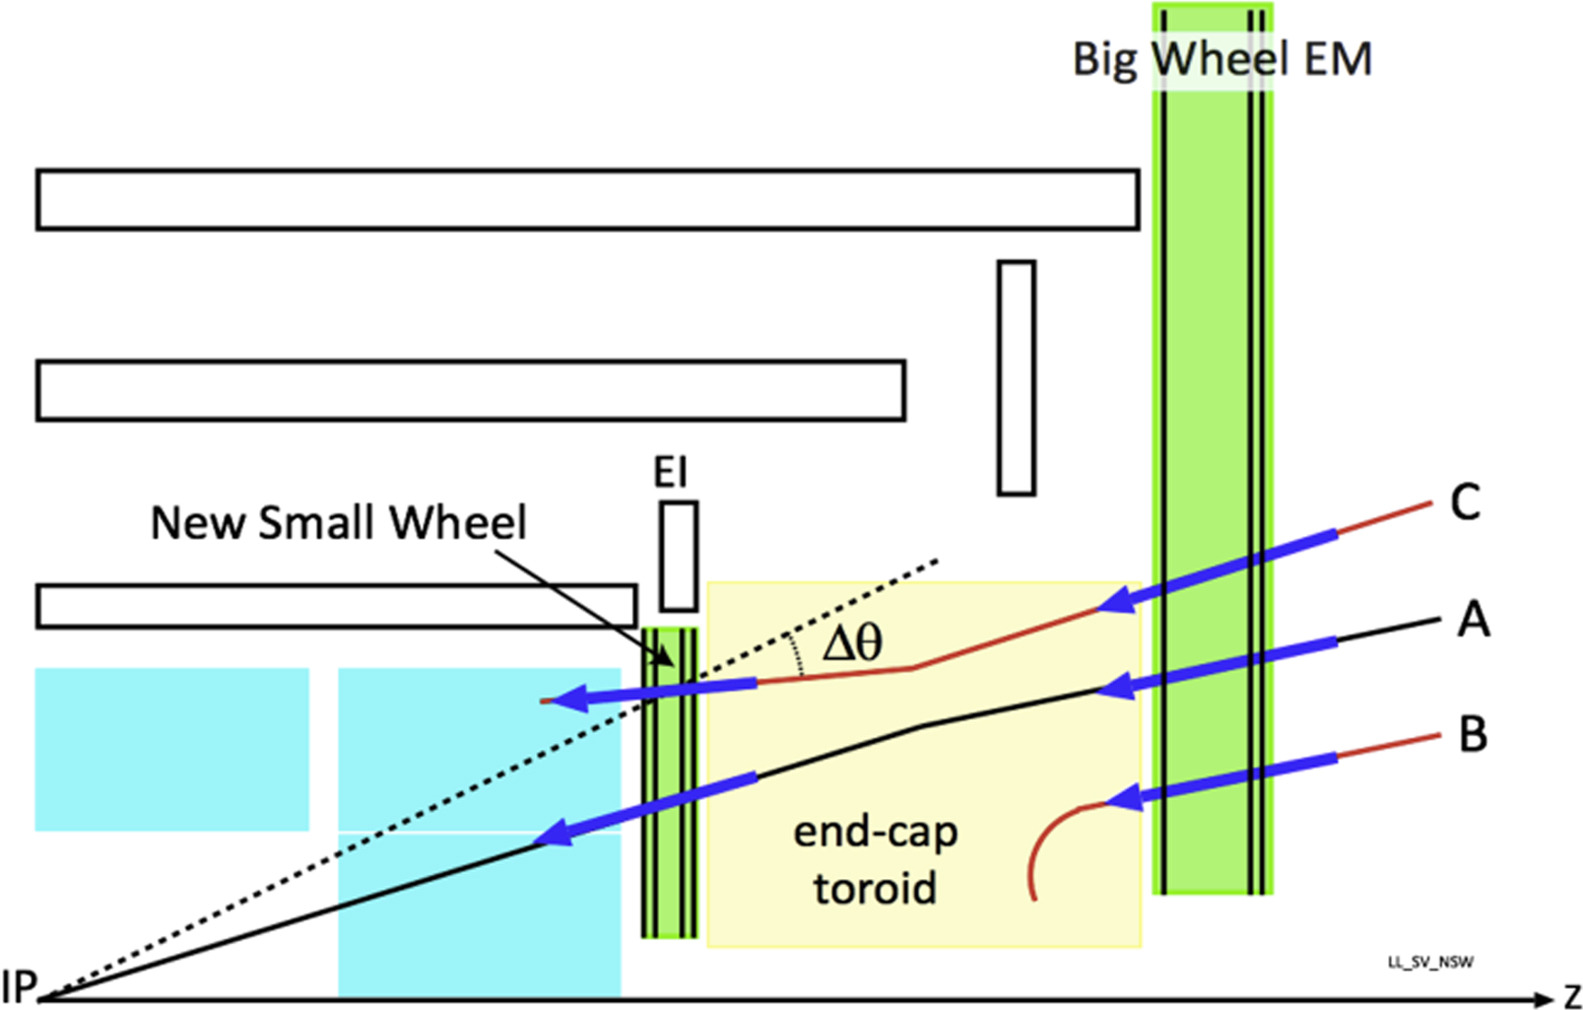
\includegraphics[width = 0.9\textwidth]{figures/perez-codina_NSW_tracks.jpg}
    \caption{A schematic of a quarter cross section of the ATLAS detector, with the collision/interaction point (IP) in the bottom left corner. Three possible tracks are labelled. Ideally, track A would be triggered upon while track B and C discarded. With the small wheel, only the big wheel provides the trigger so all three tracks would be recorded. With the new small wheel, only track A would be recorded~\cite{nsw_tdr}.}
    \label{fig:nsw_track_triggering}
\end{figure}

% --------------------------------------------------
\section{Design of the NSWs}
% --------------------------------------------------

The NSWs are covered with two detector technologies: micromegas (MM) and small-strip thin gap chambers (sTGCs). MMs are the primary tracking detectors and sTGCs are the primary triggering detectors, but for redundancy sake both are designed to do either. As such, both sets of detectors are to have better than $\sim$\SI{100}{\micro\meter} per plane. Four layered chambers of each type create quadruplet modules. Quadruplets of different sizes are assembled into wedges. Two sTGC wedges and two MM wedges are layered to create sectors (with the sTGC wedges on the outside). Sectors covered the wheel, as shown in figure~\ref{fig:nsw_diagram}. Practically, two different wedge sizes, small and large, were required to completely cover the wheel.
\begin{figure}
    \centering
    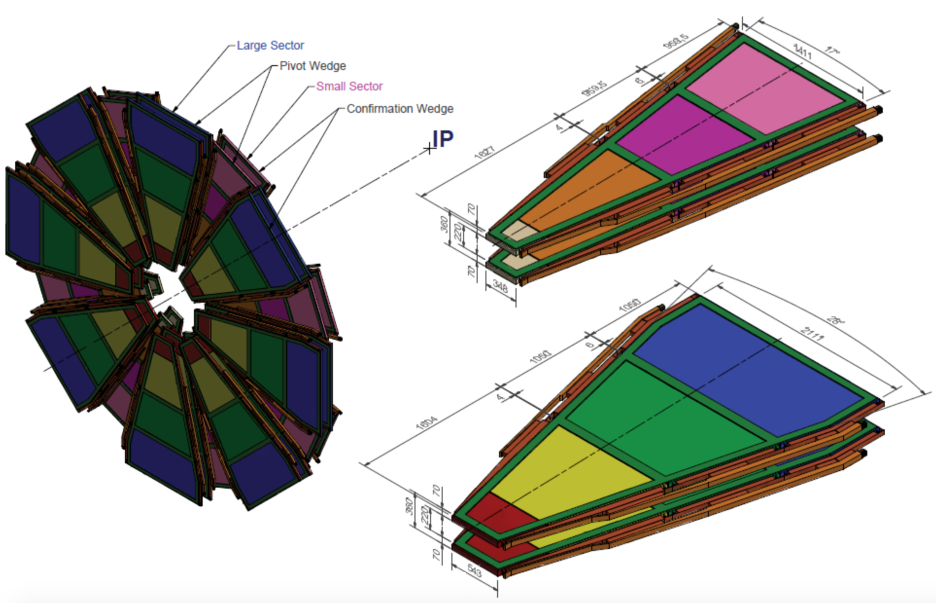
\includegraphics[width = 0.9\textwidth]{figures/nsw_diagram.png}
    \caption{Drawing of the new small wheel, and diagrams of the individual small and large wedges. Each colour represents a different sTGC module size.}
    \label{fig:nsw_diagram}
\end{figure}

\begin{figure}
\centering
\begin{subfigure}{\textwidth}
  \centering
  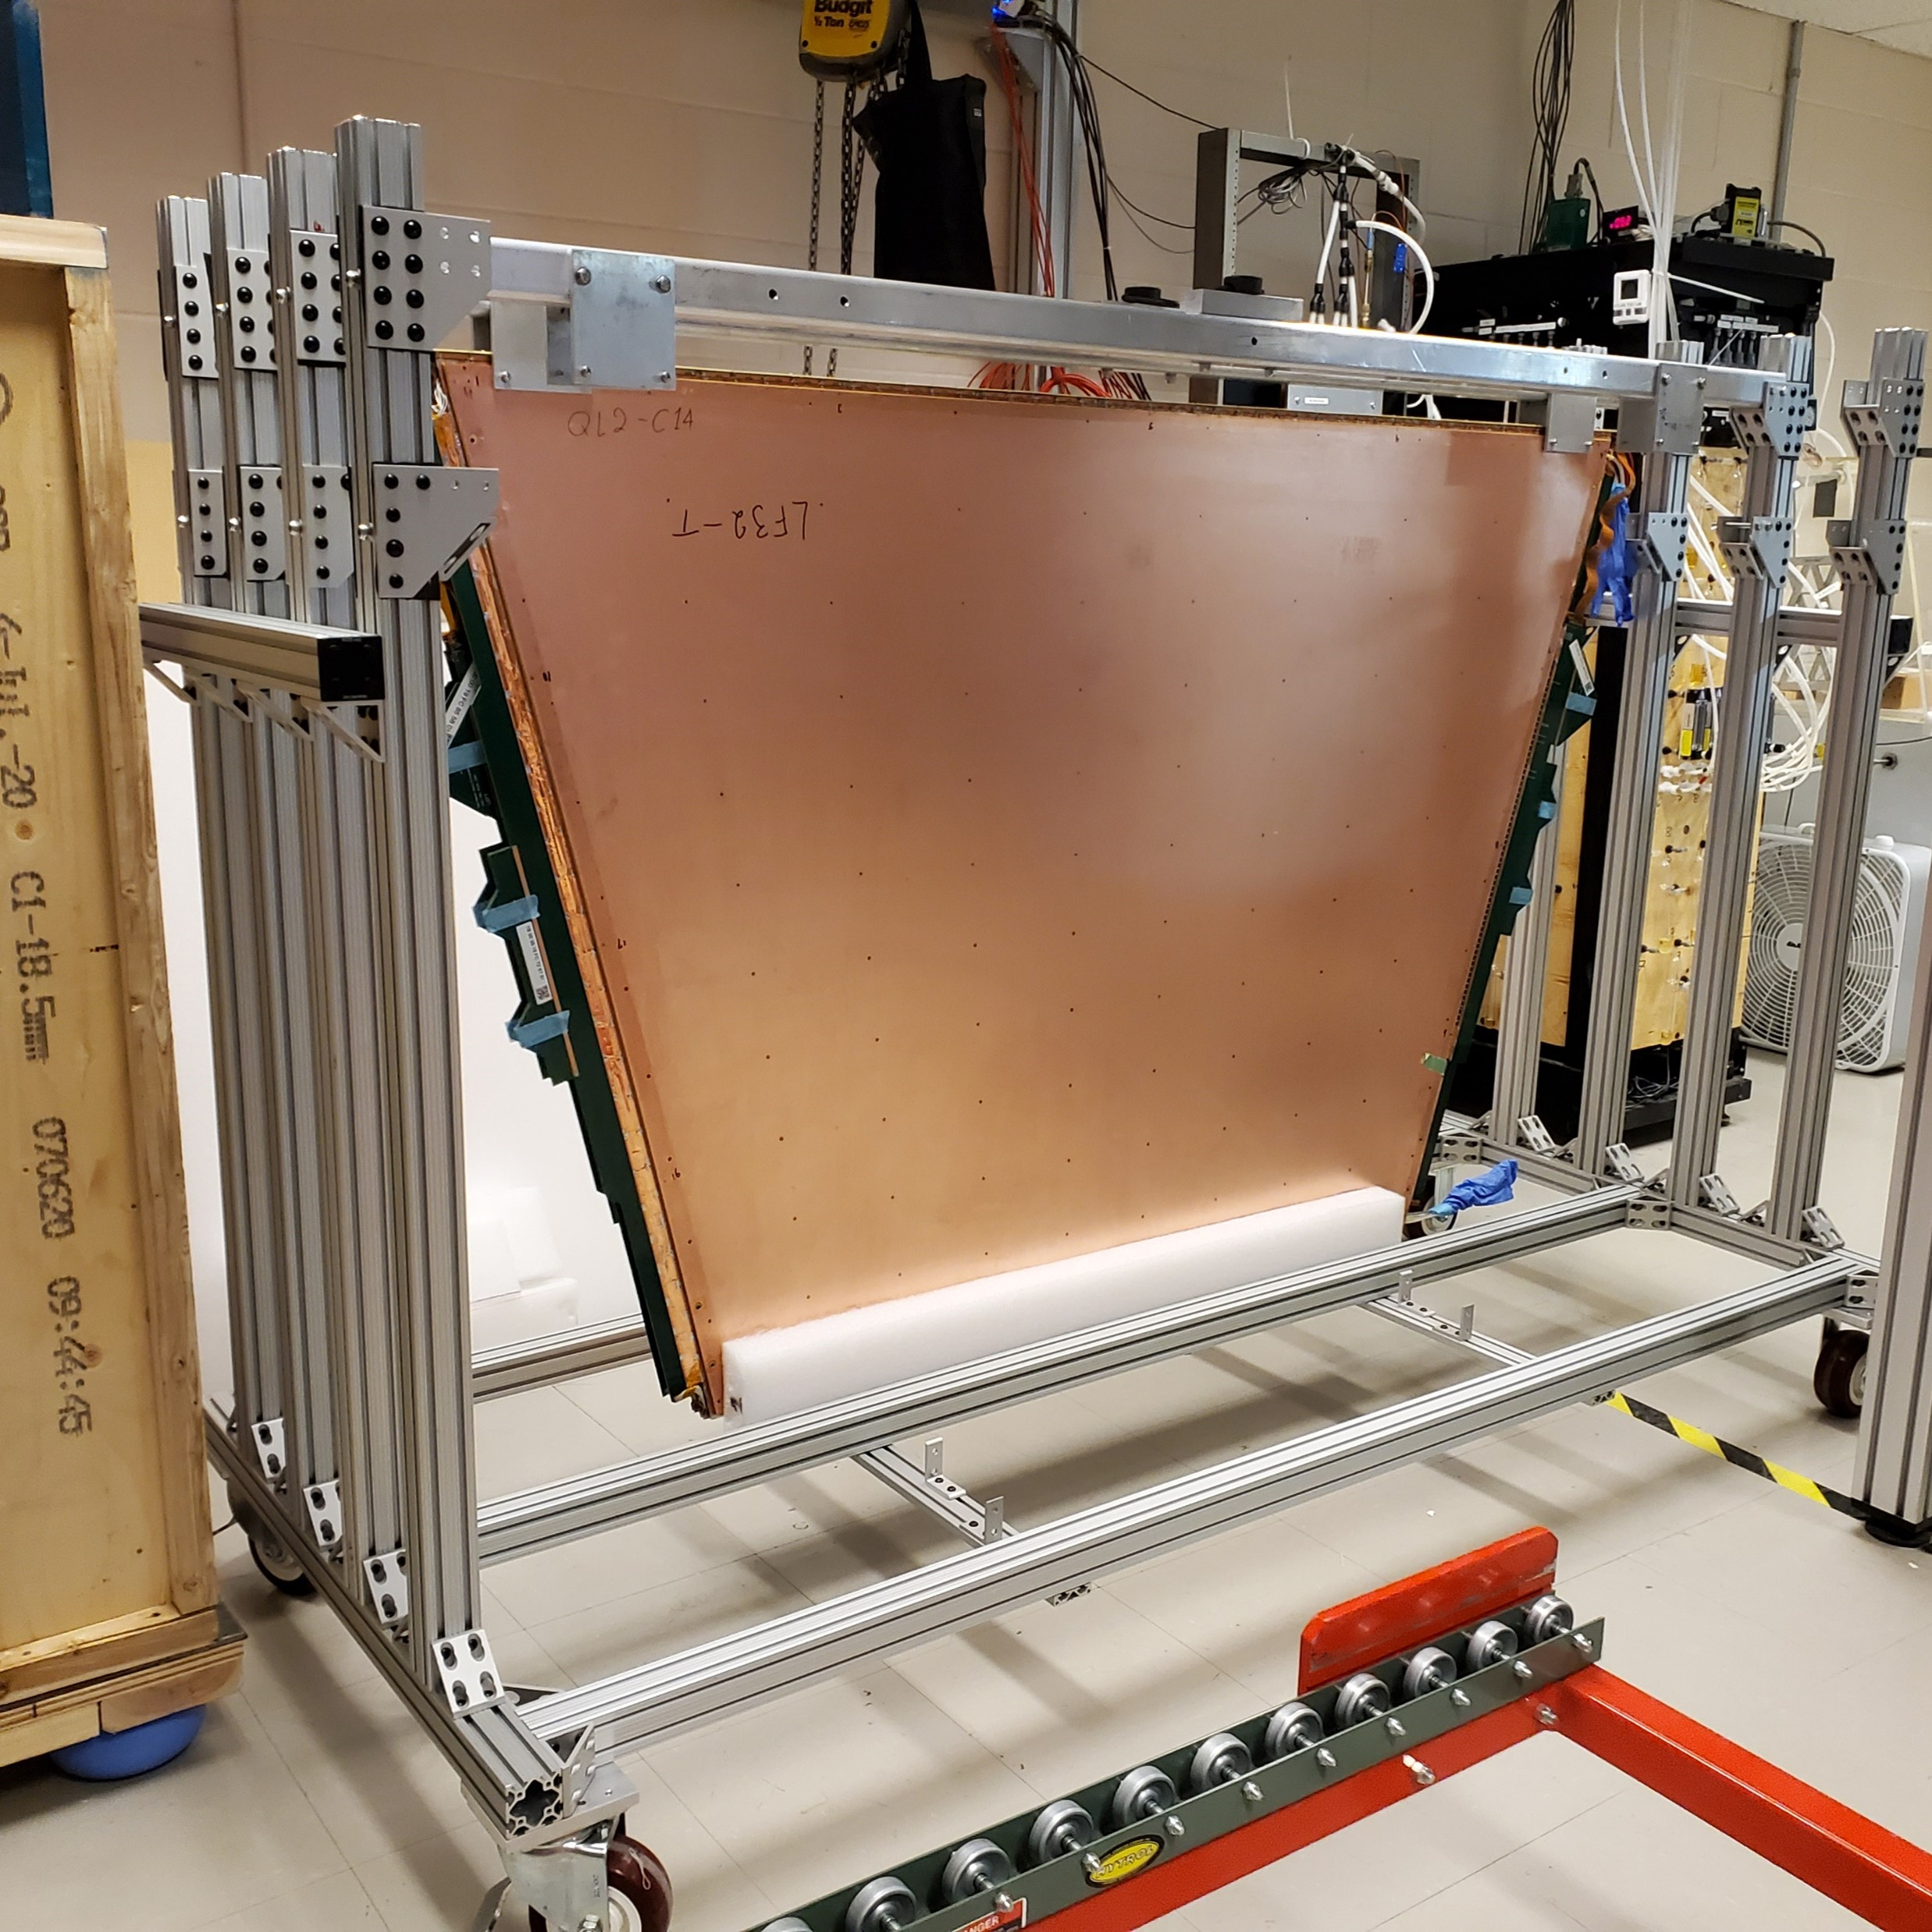
\includegraphics[width=0.4\textwidth]{figures/stgc_quad_cart.jpg}
  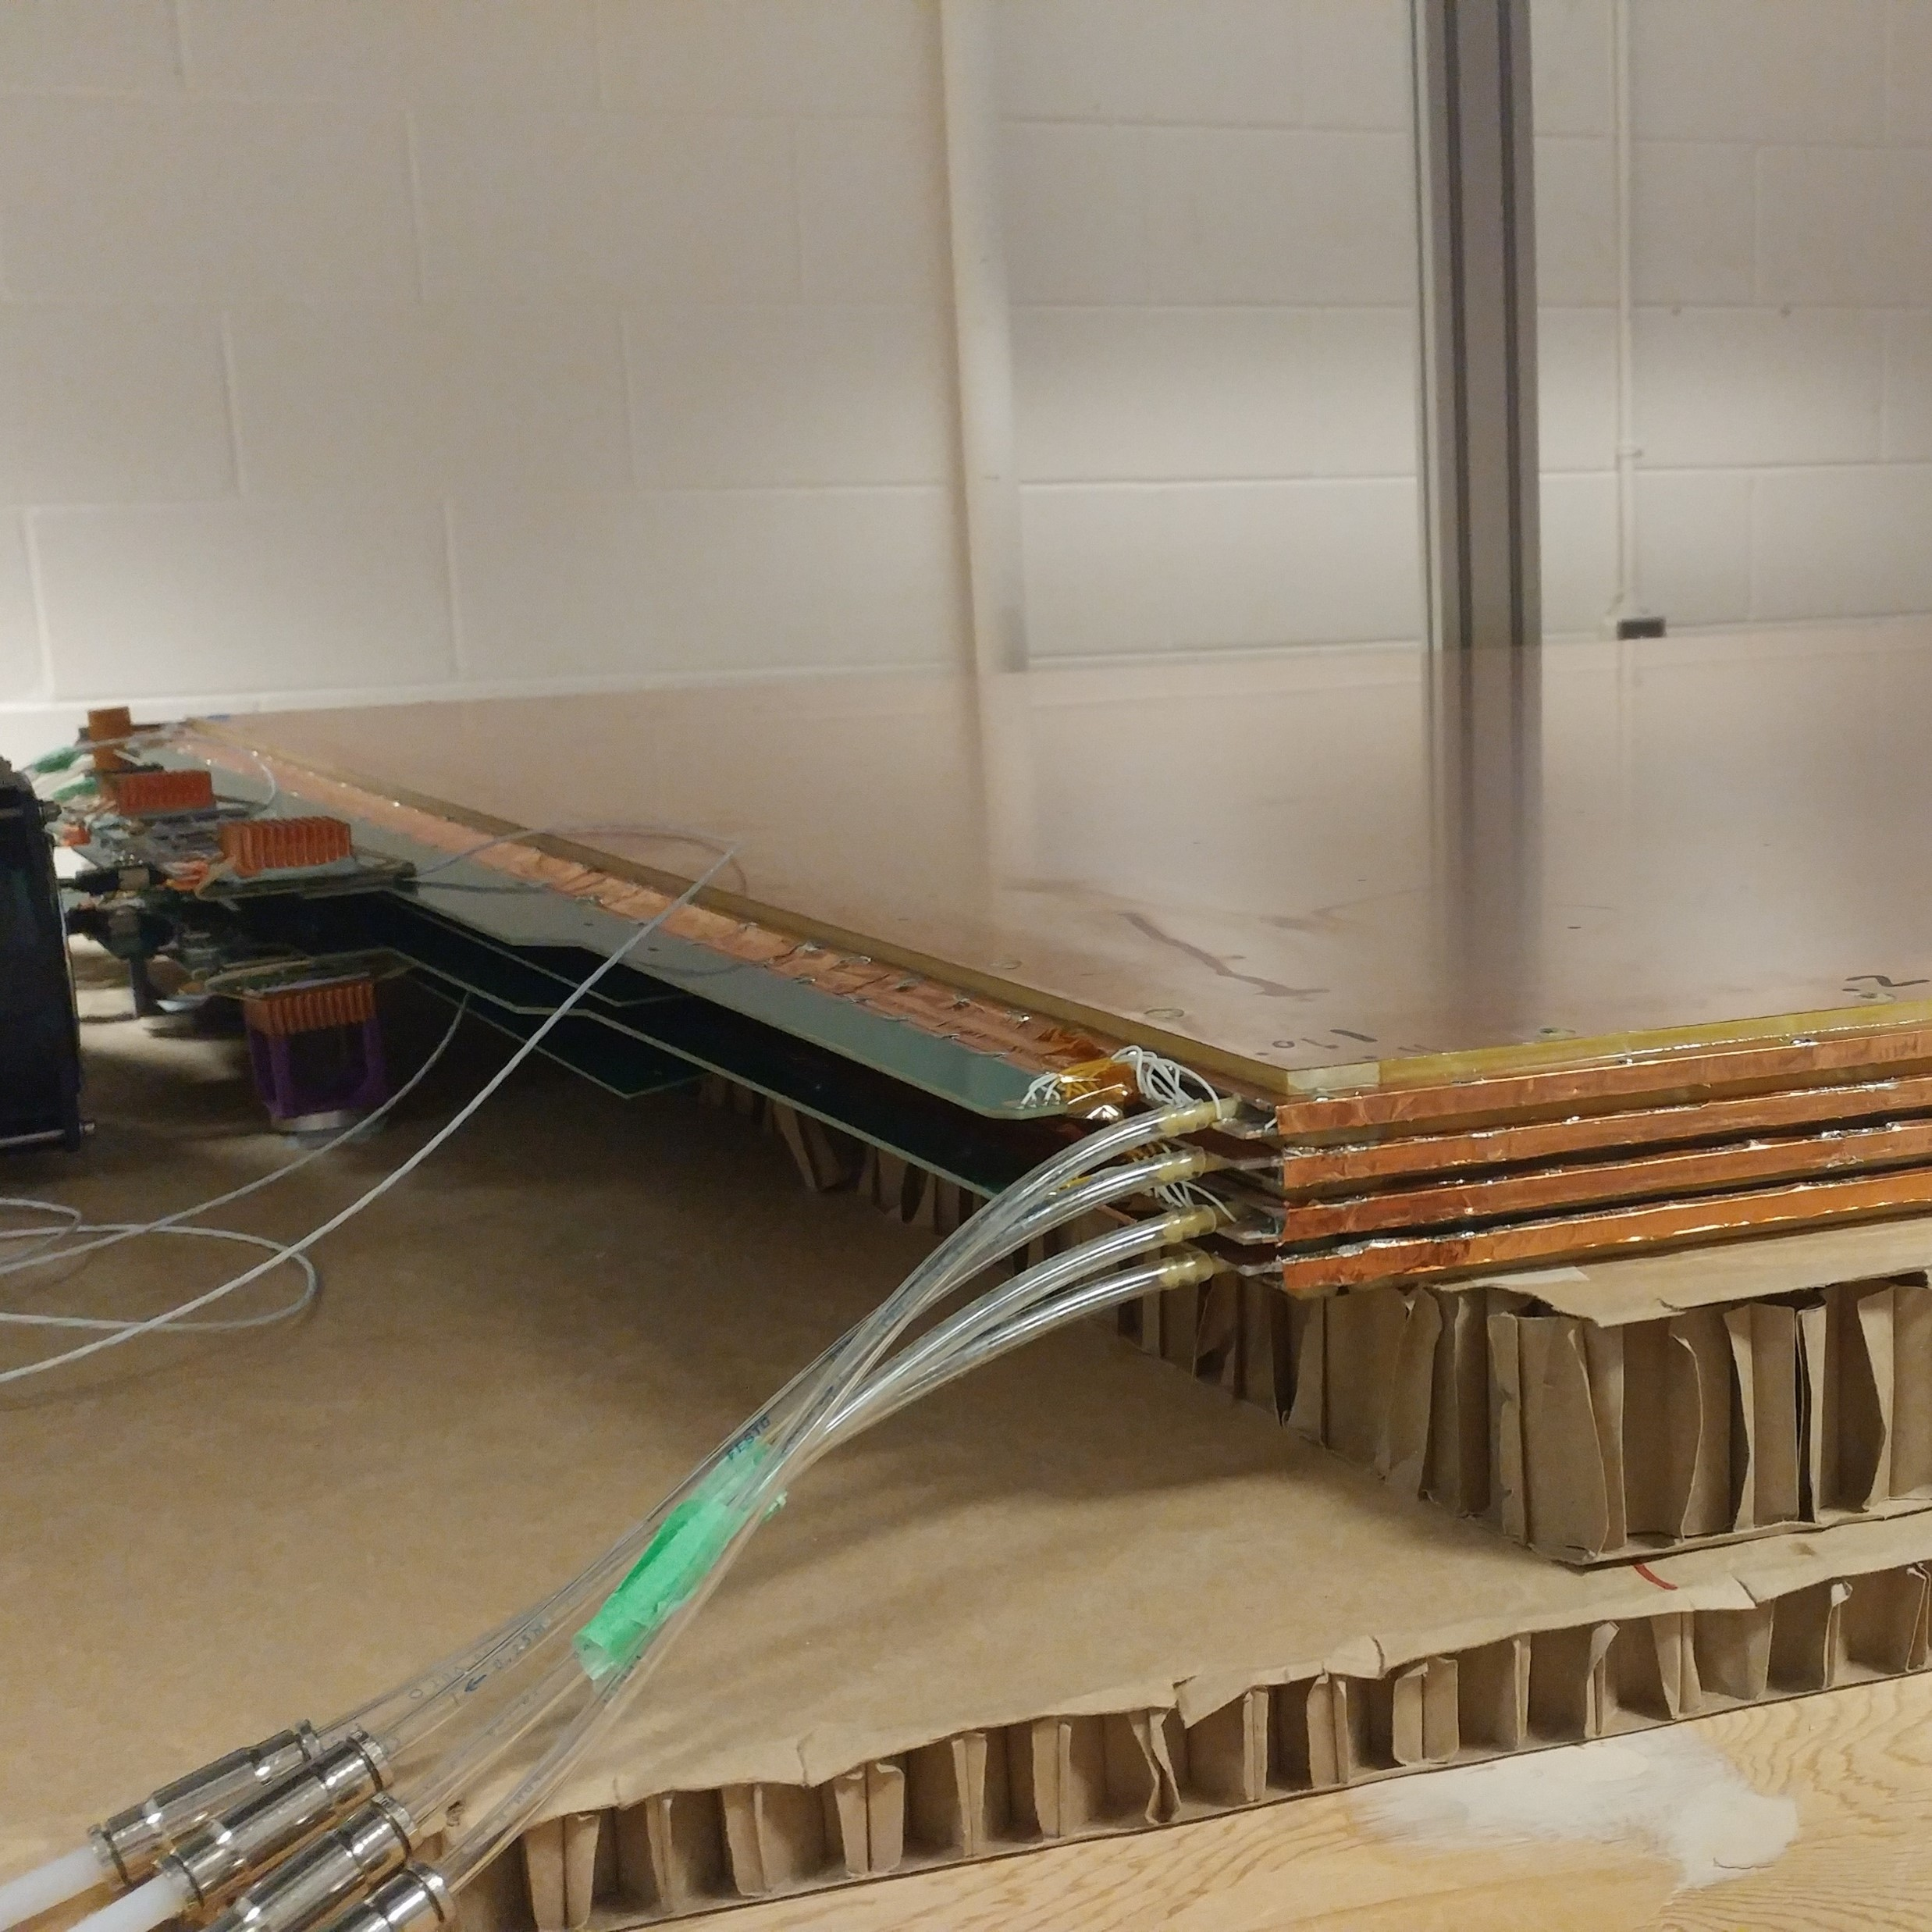
\includegraphics[width=0.4\textwidth]{figures/stgc_quad_inlet_corner.jpg}
  \caption{Individual sTGC quadruplet modules. The right image shows the short edge corner, and shows the 4 sTGC layers and the invidual gas inlets. The gas outlets and high voltage cables are at the long edge in the back of the photo.}
  \label{fig:stgc_quad}
\end{subfigure}

\medskip

\begin{subfigure}{\textwidth}
  \centering
  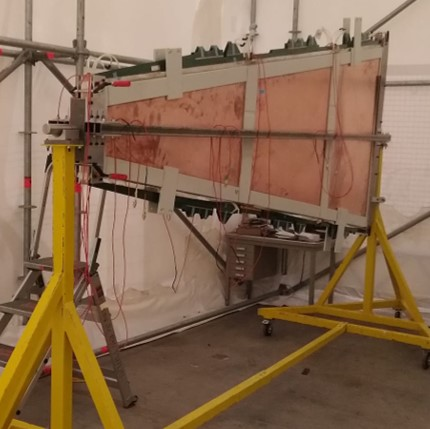
\includegraphics[width=0.4\textwidth]{figures/stgc_wedge.jpg}
  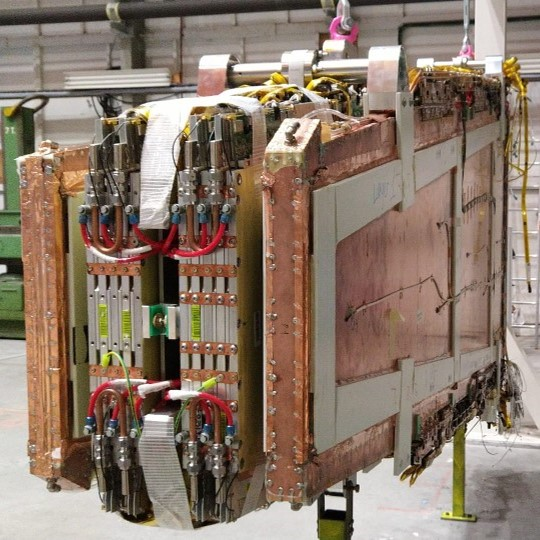
\includegraphics[width=0.4\textwidth]{figures/sector.jpg}
  \caption{Left: An sTGC wedge. The white fibreglass frame outlines the individual quadruplet modules. Right: A completed sector, with layers sTGC wedge, MM wedge, MM wedge, sTGC wedge.}
  \label{fig:wedge_and_sector}
\end{subfigure}

\medskip

\begin{subfigure}{\textwidth}
  \centering
  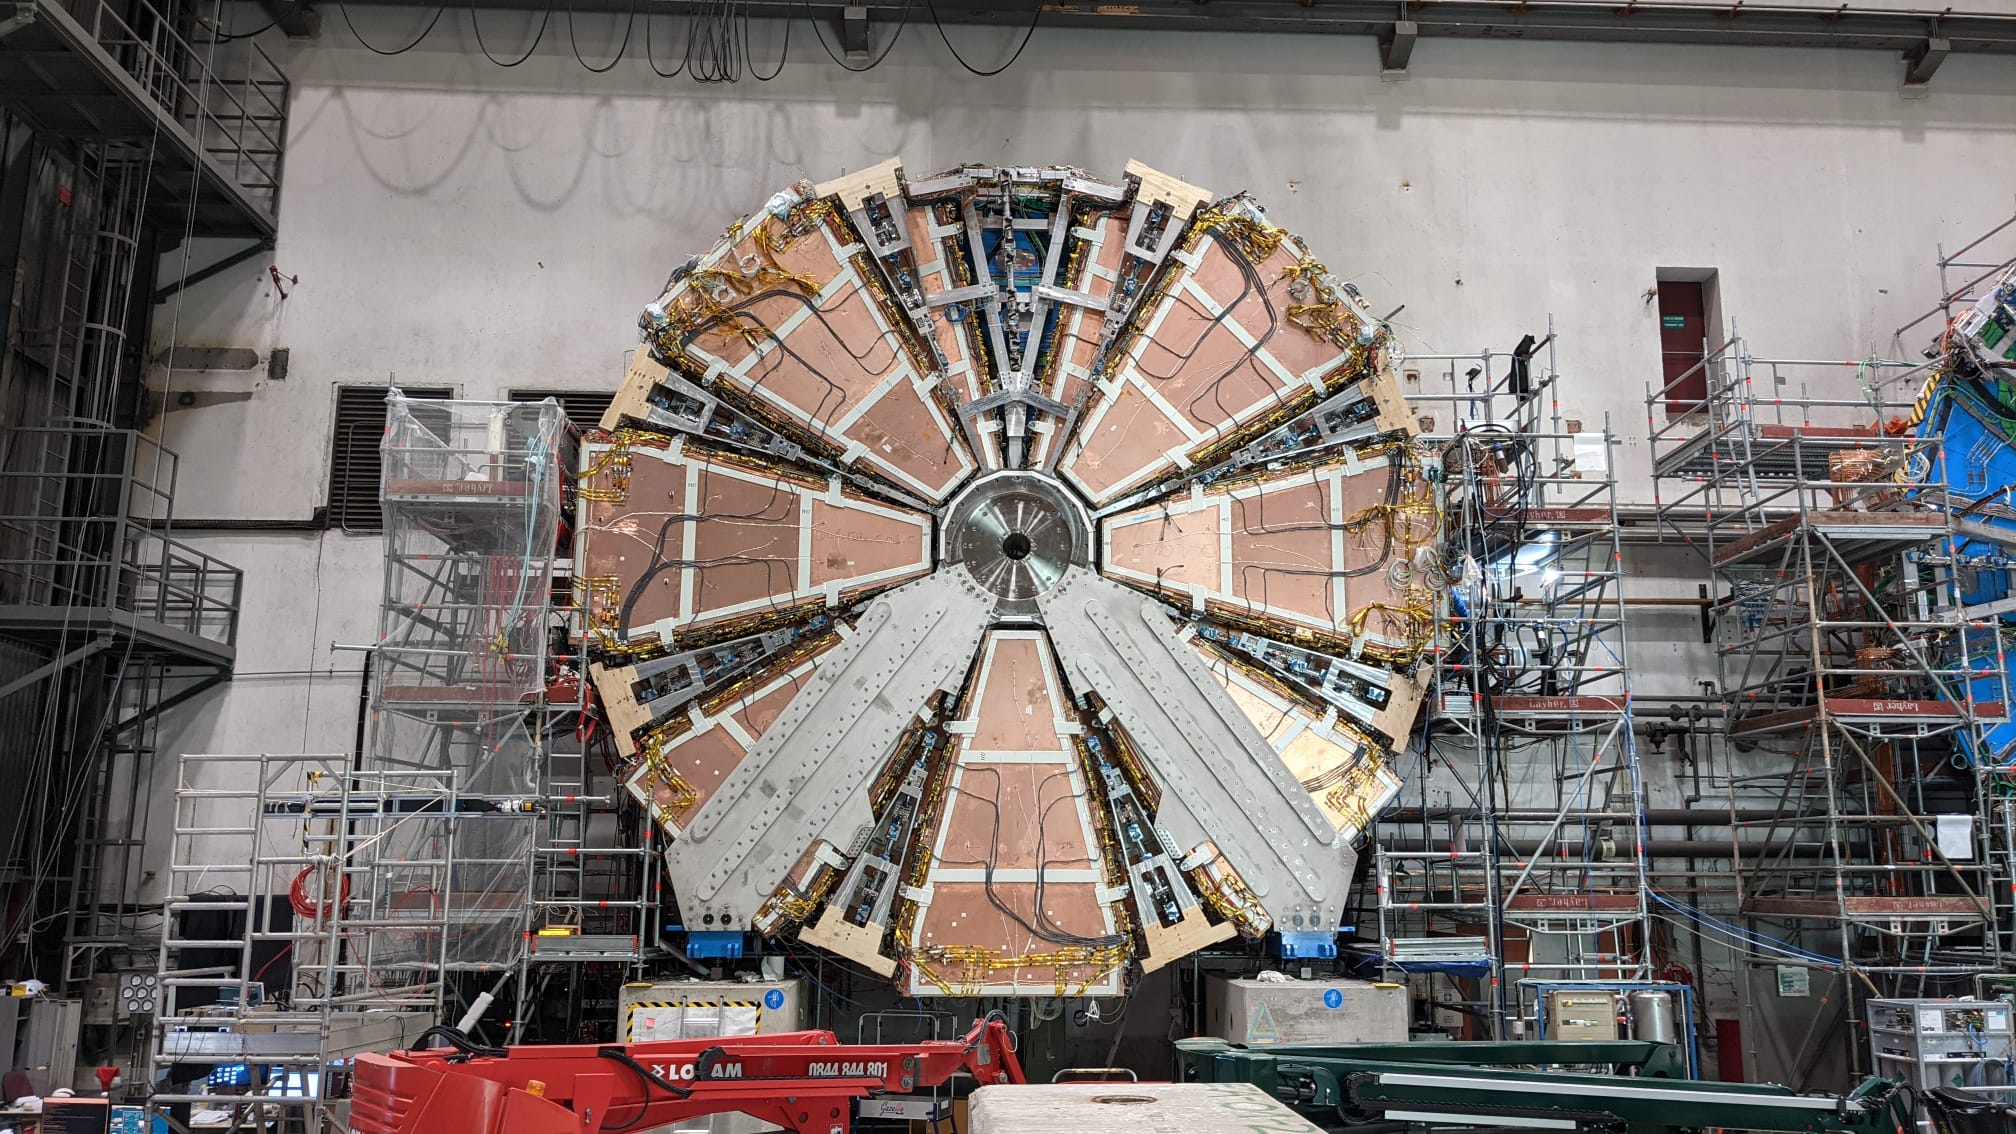
\includegraphics[width=0.8\textwidth]{figures/nsw_2021-05-27_landscape.jpeg}
  \caption{The new small wheel. All sectors except one large sector at the top are installed, revealing two of the smaller sectors that are hidden under the large sectors.}
  \label{fig:nsw}
  \end{subfigure}
\caption{Images breaking down some of the construction units of the NSWs.}
\label{fig:nsw_breakdown}
\end{figure}

For the tracking and triggering goals, each chamber must have a position resolution of $\sim$\SI{100}{\micro\meter}. 

%TODO : Pivot vs confirm?

% --------------------------------------------------
\section{Micromegas}
% --------------------------------------------------

Micromegas have three components: a drift plane, a gas gap, a mesh, and readout strips, as shown in figure~\ref{fig:micromega}. High voltage is applied to the readout strips. An ionization event in the gas causes electrons to drift towards the mesh. Once they arrived, they are amplified by the strong field and the avalanche is picked up by the readout electrodes. The small distance between the readout electrodes and the mesh, \SI{128}{\micro\meter}, means that positive ions are evacuated in $\sim$\SI{100}{\nano\second}, making micromegas a good choice for high rate environments~\cite{nsw_tdr}. The small pitch of the readout electrodes, \SI{0.425}{mm} provide spatial resolution better than \SI{100}{\micro\meter}~\cite{stelzer_new_2016}.

\begin{figure}
    \centering
    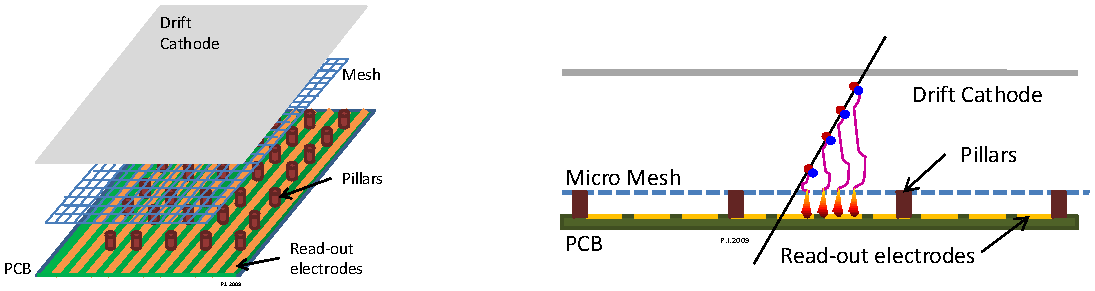
\includegraphics[width = 0.9\textwidth]{figures/micromegas.png}
    \caption{Sketch the micromega operating principle. Positive high voltage is applied to the readout electrodes, which creates a strong field between the mesh and the readout electrodes, and a weaker field between the mesh and the drift cathode. Amplification takes place between the readout electrodes and the mesh. }
    \label{fig:micromega}
\end{figure}

Four micromega modules will be layered to form a quadruplet, then two quadruplets of different sizes form a wedge. The muon position provided by each of the four layers will provide the NSW precision tracking information~\cite{nsw_tdr}.

% --------------------------------------------------
\section{Small-strip thin gap chambers}
% --------------------------------------------------

sTGCs are gas ionization chambers operated with a CO$_2$:n-pentane ratio of 55:45. Gold-plated tungsten wires of \SI{50}{\micro\meter} in diameter are suspended in the plane with \SI{1.8}{mm} is suspended between two cathode planes made of FR-4, \SI{1.4}{mm} each away. One cathode board is segmented into pads of varying area (around \SI{300}{cm^2}), and the other segmented into strips of \SI{3.2}{mm} pitch, perpendicular to the wires. High voltage is applied to the wires and the cathode planes are grounded. When a muon passes through, the gas is ionized and the electric field in the gas gap causes an ionization avalanche~\cite{townsend_electricity_1915}. The motion of the ions and electrons are picked up on the nearby wire, strip and pad electrodes. The hatching of the strips and wires establishes a coordinate system from which to extract the coordinate of the muon as it passes through the layer. Signal is readout from groups of successive wires, so the position resolution in the direction perpendicular to the wires is $\sim$\SI{10}{mm}. The resolution in this direction does not matter since it will give the symmetric azimuthal coordinate in ATLAS. Good resolution on the $\eta$ coordinate is important, which is the direction perpendicular to the strips. The average single chamber position resolution in the strip coordinate was \SI{45}{\micro\meter} measured for perpendicular muon tracks in a test beam~\cite{abusleme_performance_2016}~--- well within design specifications. When four sTGCs are glued together into a quadruplet the design angular resolution of ~\SI{1}{mrad} in the strip coordinate is achievable~\cite{nsw_tdr, perez-codina_small-strip_2016}.

A 3-out-of-4 coincidence in the pad electrodes of a quadruplet will define a region of interest where the strip and wire electrodes should be readout~\cite{nsw_tdr}. Then, a track segment with the required angular resolution can be constructed and provided as input to the L1 trigger~\cite{tdaq_phase1_tdr}. For run 3, the L1 trigger will pass if the track segment from the small wheel matches a region of interest defined by the TGCs of the big wheel. The increased angular resolution and $\eta$ coverage of the quadruplets will be an improvement in the triggering scheme over the current SW TGCs. After the phase II upgrade of the trigger and data acquisition system, which includes upgrades to the big wheel's angular resolution, there will only be a trigger if the combined track points back to the interaction point, increasing the muon $p_T$ resolution~\cite{tdaq_phase2_tdr}.

% Maybe put NSW alignment system next, then go into construction and misalignment. This paragraph can go after section on NSW alignment system.
The original design goal was to position the strips within \SI{40}{\micro\meter} per detector plane. This was necessary to ensure that the position reconstruction would be unbiased when the quadruplets are installed in ATLAS, allowing the quadruplets to deliver the design angular resolution. The NSW alignment system will monitor the surface of the sTGC wedges (discussed \textcolor{red}{LATER}) so the internal alignment of the chambers had to be controlled during construction or quantified before installation. The main alignment feature of the strip cathode boards were brass inserts along one of their angled edges, near the long edge and short edge. These inserts accessible outside the gas gap throughout the construction process, and were meant to provide an external reference from which to measure the position of internal components of the chambers. The brass inserts on a quadruplet are visible in figure~\ref{fig:brasses}. The process of sTGC construction is highlighted in section~\ref{sec:stgc_construction}, with steps important to alignment highlighted.

% In addition, the sTGC quadruplets should be able to provide precision tracking within \SI{100}{\micro\meter} per plane in the event of a MM module failure.

\begin{figure}
\centering
\begin{subfigure}{.5\textwidth}
  \centering
  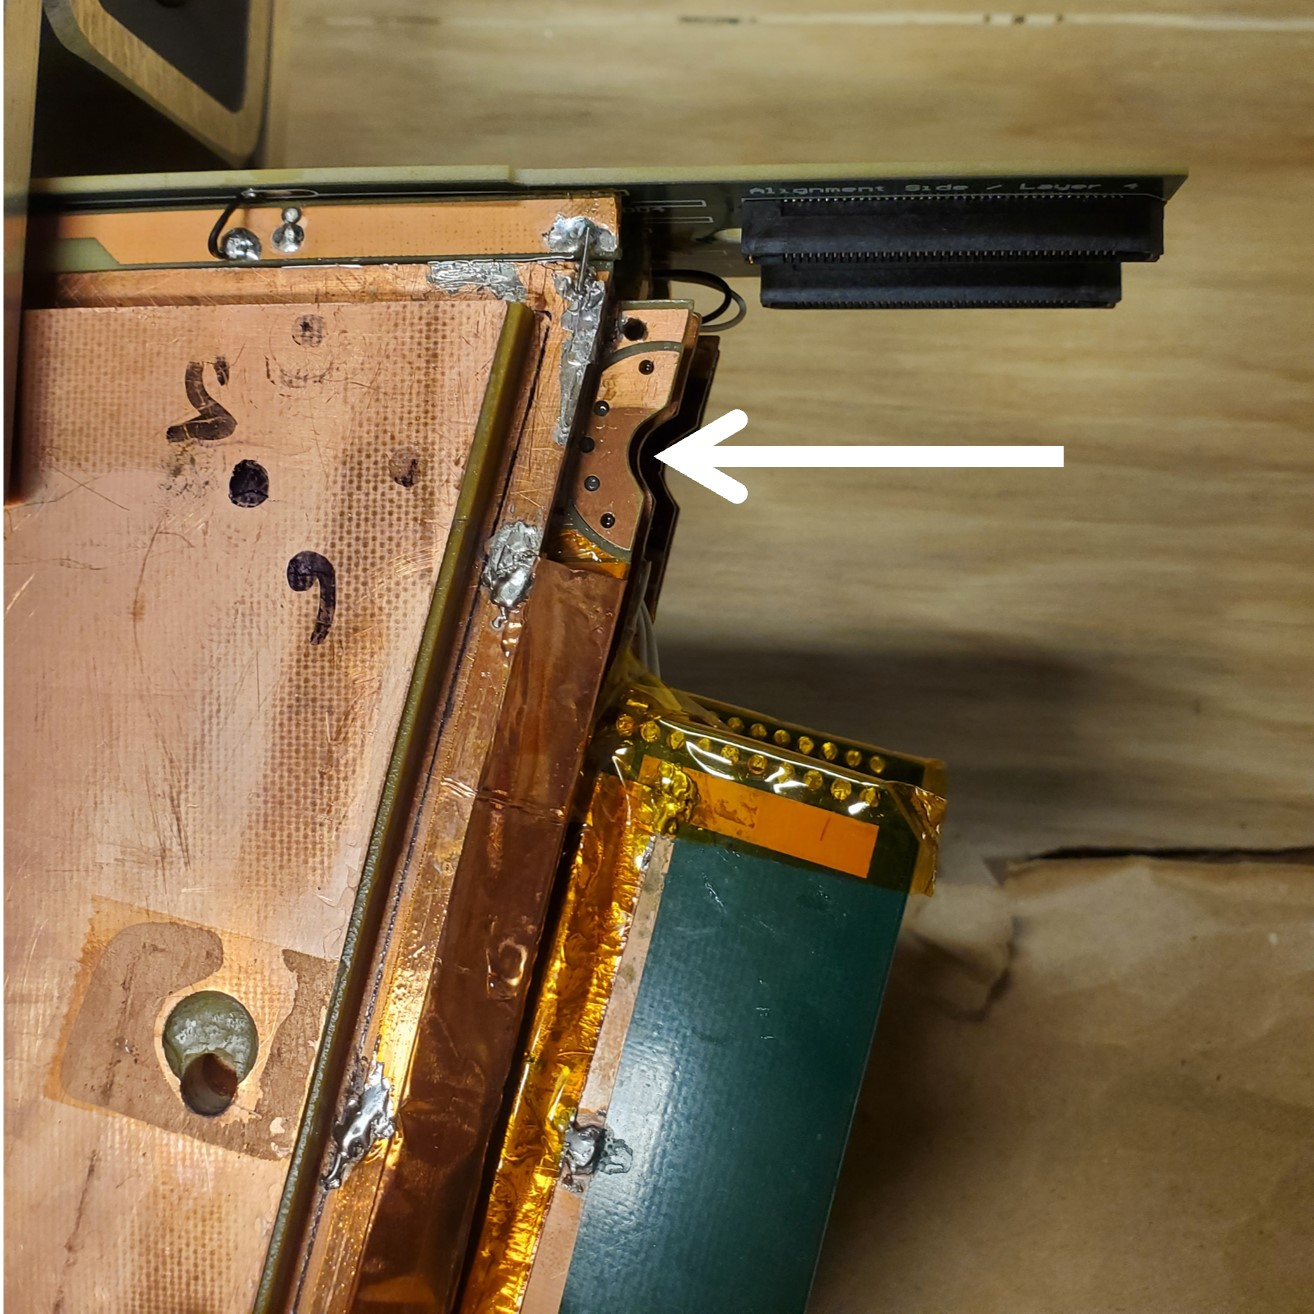
\includegraphics[width=\linewidth]{figures/brass_top.jpg}
  \caption{Brass insert near long edge.}
  \label{fig:brass_top}
\end{subfigure}%
\begin{subfigure}{.5\textwidth}
  \centering
  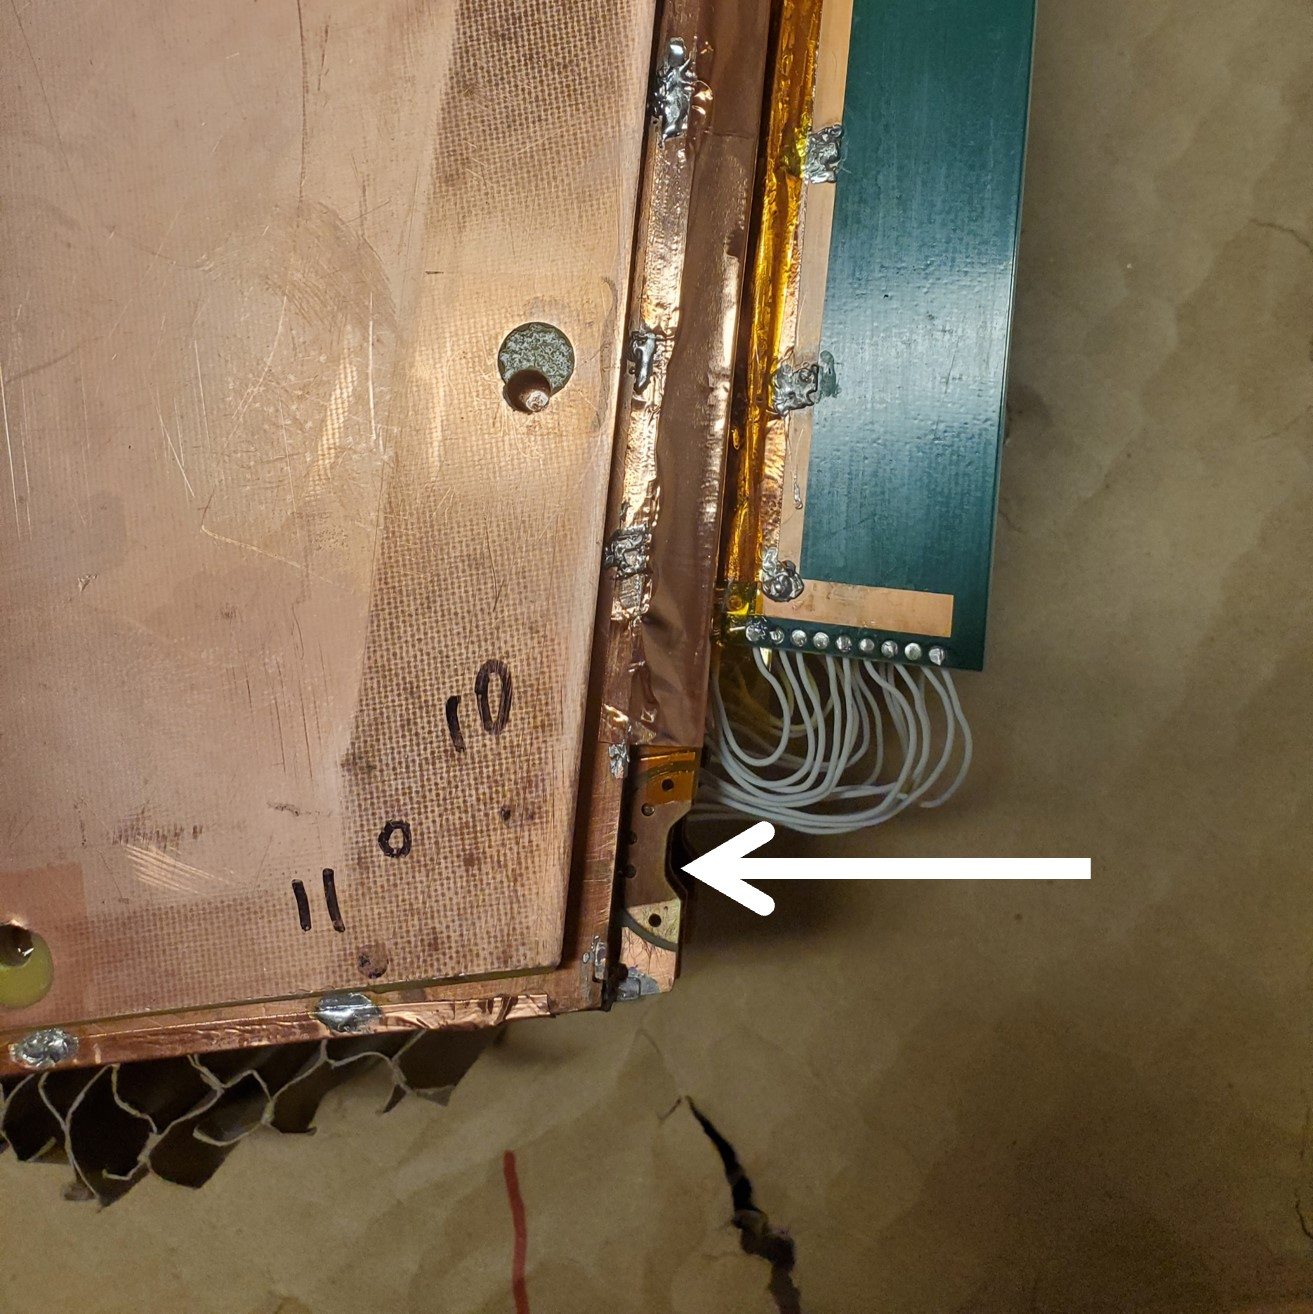
\includegraphics[width=\linewidth]{figures/brass_bottom.jpg}
  \caption{Brass insert near short edge.}
  \label{fig:brass_bottom}
\end{subfigure}
\caption{The brass inserts sticking out from the gas volumes of an sTGC quadruplet (from a bird's eye view). These inserts were pressed against alignment pins when the individual sTGCs were being glued together.}
\label{fig:brasses}
\end{figure}

% --------------------------------------------------
\section{sTGC Quadruplet Construction}
% --------------------------------------------------
\label{sec:stgc_construction}

Five countries were responsible for producing the sTGC modules of varying geometries for the NSW: Canada, Chile, China, Israel and Russia. Canada was responsible for 1/4 of the required sTGCs, of three different geometries. The steps of the construction process in each country were similar. The process followed in Canada is detailed in this section.

The cathode boards were prepared at a commercial industry. They are multilayer boards made of FR-4, but the strip boards required precision machining to etch the strip pattern and install the brass inserts~\cite{nsw_tdr}. Two sources of misalignment resulted at board level: the placement and shape of the brass inserts could be imperfect and there could be non-conformities in the strip pattern. Carlson addressed and measured the non-conformities in the strip pattern of Canadian cathode boards in his thesis~\cite{carlson_results_2019}. A coordinate measuring machine (CMM) or FaroArm was used to measure non-conformities in the strip pattern, and the results are available on a QA/QC database. Non-conformities included an offset and rotation, plus some higher order deformations. It is common, however, for alignment models to only consider an offset and rotation. Tracking accuracy not affected by micrometer-level non-conformities in the pad pattern so it is not of concern.
% Do I need to define elongation, non-parallelism?

Once the cathode boards were created, they were sent to TRIUMF in Vancouver, British Columbia to be sprayed with the graphite coating. After spraying, the coating was polished until the resistivity was between 90 and \SI{110}{\kilo\ohm}$/\msquare$, then wire support structures and frames were installed~\cite{nsw_tdr}. The completed boards were sent to Carleton university for construction into gas gaps and multiplets.

First, anode wires are wound onto the the pad cathode boards using a rotating vacuum table. Then, the wires are soldered in place. Gluing is done with the cathode boards held in place by vacuum on a flat (within \SI{20}{\micro\meter}) granite table. To create a gas gap, a wired-pad board is held in place on a vacuum table and a strip board glued on top~\cite{nsw_tdr}. Any relative misalignment of the pad board with respect to the strip board is not significant since the pad does not provide precision coordinates. Half a layer of honeycomb spacer is glued on top of each singlet. Two brasses of the strip boards of two singlets are pushed against alignment pins and glued to create a doublet. In the same way, two doublets can be glued into a quadruplet. The position of the brasses are recorded in 3D using an x-ray gun~\cite{nsw_tdr}. Also, the alignment between strips visible outside the gas gap is checked with a microscope~\cite{carlson_results_2019}. Once a quadruplet is glued, adapator boards used to route the electrodes to the front end electronics are soldered on to the angled sides of the quadruplet~\cite{nsw_tdr}. 

Quality control tests of alignment, ability to hold high voltage, gas sealing etc. were undertaken at every stage in the construction process, the details of which can be found in~\cite{nsw_tdr}. The final set of quality control and characterization was done at McGill University in Montreal, Quebec. Completed quadruplets were tested for gas leaks, the noise of the electrodes measured, and finally characterized with cosmic rays. The details of cosmic ray testing are described in chapter~\ref{chap:cosmics}.

% --------------------------------------------------
\section{NSW alignment}
% --------------------------------------------------

Once the quadruplets have been tested with cosmics rays, they are sent to CERN to be further tested, assembled into wedges then sectors, then installed on the NSWs. 

The idea of the NSW alignment system is presented in~\cite{nsw_tdr}, but the details have only been presented internally so far. The original goal of the alignment system was to provide the position with respect to one another of any three chambers traversable by a muon track with an accuracy of \SI{40}{\micro\meter} in the precision coordinate~\cite{nsw_tdr}. Likely for sTGCs, this will mean inputing the strip postions, or parameters to calculate the strip positions, into the ATLAS experiment's offline software, \package{Athena}.

%TODO : 
\textcolor{red}{What figures can I use to show the bars, the alignment jig, the platforms and the optical fibres?}.
After the wedges are constructed, alignment platforms are installed on every sTGC quadruplet and optical fibres routed to them. They are positioned with the help of an alignment jig, which is like a frame that can be positioned on top of a wedge with cut outs indicating the correct position for the alignment platforms. The jig is positioned with respect to the brass inserts \textcolor{red}{[Benoit 2020-01-20, 2020-04-16 presentations]}.  Light from the optical fibres will be monitored in real time by cameras (BCAMs) mounted on the alignment bars of the new small wheel. The system will thus record the positions of the alignment platforms in the ATLAS coordinate system, accessible at any point during operation \textcolor{red}{Camila Pazos, 2021-02-01 and Chris Armstrong 2021-02-02 during muon weekb https://indico.cern.ch/event/983500/}. The final link in the sTGC alignment system requires knowing the position of the strips inside a chamber with respect to the alignment platforms.

The goal was to control the position of the strips in the chamber to within ~\SI{40}{\micro\meter} for precision tracking goals~\cite{nsw_tdr} --- then knowing the position of the brass inserts with respect to the alignment platforms would allow the strips to be positioned sufficiently. That is the alignment scheme shown in solid arrows in figure~\ref{fig:alignment_elements}. Due to time constraints, tolerances on the non-conformities in the etched strip pattern were loosened, with the condition that the strips positions would have to be corrected for in the software~\cite{carlson_results_2019}. Then, non-conformities in the brass inserts, misalignment of the pins the brass inserts were pushed against, and shifts of the strip layers while the glue was curing resulted in misalignments between the brass inserts and the strips layers that prevent using the brasses as an external reference of the position of the strips. The misalignments between Canadian sTGCs were shown to be random~\cite{carlson_results_2019}, so no one correction would suffice.

\begin{figure}
    \centering
    
\includegraphics[width = 0.9\textwidth]{figures/alignment_system_element_relations.png}
    \caption{How the different elements of the sTGC alignment system relate to one another. The solid arrows denote the planned alignment scheme. The dashed arrow shows the modification being finalized now. This figure is based off of \textcolor{red}{Benoit's presentation, 2021-01-30.}}
    \label{fig:alignment_elements}
\end{figure}

A different method to get the position of the individual strips with respect to the alignment platform is currently in its final stages. It uses the quadruplet characterization datasets~-- cosmic muon, CMM, and the yet unmentioned x-ray datasets~-- to calculate the offsets in the strip pattern in a local area (local strip pattern offsets). Effectively, the reference to the brass inserts is skipped, represented as the dashed line in figure~\ref{fig:alignment_elements}. The goal of this thesis is to validate the x-ray local strip pattern offsets with cosmic muon data. In chapter~\ref{chap:cosmics}, how cosmic muon data collection and processing is done at McGill University is presented. Chapter~\ref{chap:cosmics_for_alignment} and \textcolor{red}{CHAPTER XRAY} detail how measurements of local strip pattern offsets are measured with cosmic muon data and x-ray data. In chapter~\ref{chap:comparison}, cosmic muon and x-ray local strip pattern offsets are compared to validate the x-ray dataset. Finally, in chapter~\ref{chap:outlook}, the context of these results in the alignment scheme is presented.

% Snippets
%The main dataset was collected using x-rays as the probe. The x-ray data has been combined with the CMM data to create an alignment model that can be used to estimate the position of each strip. The goal of this work was to validate the measurements of strip pattern offsets done with the x-ray dataset with the cosmic muon data. Currently, only modules made in Canada have been analyzed in this way, but the method applies for other countries that were able to collect cosmic muon data on multiple quadruplet layers. 

%Moreover, as-built alignment parameters must be measured and extracted to ensure proper function and provide a way to correct for misalignment. The next section breaks down the sTGC construction process to highlight the stages of alignment.
%All countries successfully finished delivering their modules this year, and the sectors have been installed on the NSWs. 






























